\begin{frame}
\begin{center}
Why aviation?
\end{center}
\end{frame}

\begin{frame}
\frametitle{Aviation}
\begin{block}{I live near here}
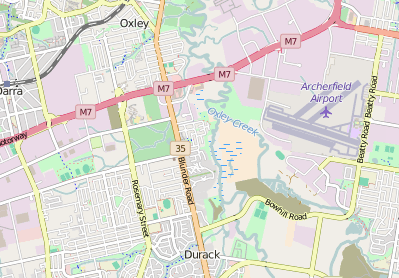
\includegraphics[height=0.5\textheight]{image/archerfield-map.png}
\end{block}
\end{frame}

\begin{frame}
\frametitle{Aviation}
\begin{block}{This is the 10L/28R circuit pattern for Archerfield (YBAF)}
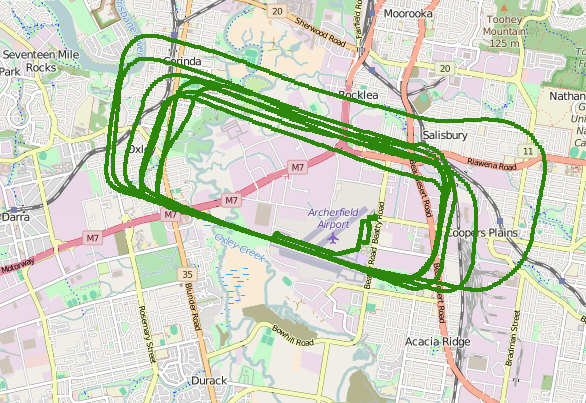
\includegraphics[height=0.5\textheight]{image/archerfield-circuit.png}
\end{block}
\end{frame}

\begin{frame}
\frametitle{Aviation}
\begin{block}{and I'd see this on my way home}
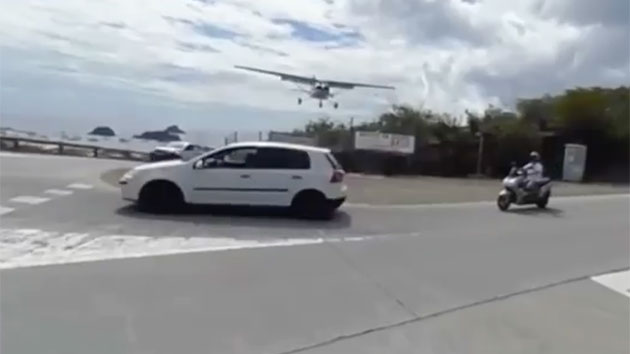
\includegraphics[height=0.5\textheight]{image/aeroplane-approach.jpg}
\end{block}
\end{frame}

\begin{frame}
\frametitle{Aviation}
\begin{block}{This is me on my way home}
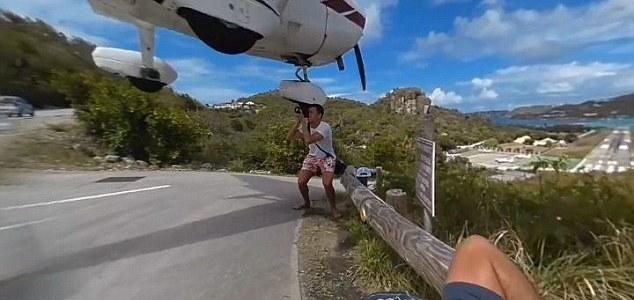
\includegraphics[height=0.5\textheight]{image/aeroplane-graze-photographer.jpg}
\end{block}
\end{frame}

\begin{frame}
\frametitle{Aviation}
\begin{block}{and so}

\includegraphics[height=0.5\textheight]{image/thought-bubble-thats-it.png}
\end{block}
\end{frame}

\begin{frame}
\frametitle{Aviation}
\begin{block}{In November 2015, I did this}

\includegraphics[height=0.5\textheight]{image/flight-school-google.png}
\end{block}
\end{frame}

\begin{frame}
\frametitle{A domestic argument ensued}
\begin{block}{My lovely wife Amanda was like}

\includegraphics[height=0.5\textheight]{image/thought-bubble-dollars.png}
\end{block}
\end{frame}

\begin{frame}
\frametitle{A compromise was reached}
\begin{block}{and I was like}

\includegraphics[height=0.3\textheight]{image/tom-cruise.png}
\end{block}
\end{frame}

\begin{frame}
\frametitle{The argument was over}
\begin{block}{and Amanda was like}

\includegraphics[height=0.5\textheight]{image/thought-bubble-good-point.png}
\end{block}
\end{frame}

\begin{frame}
\frametitle{Pilot Licences}
\begin{block}{There are (loosely) four levels of CASA pilot licence}
\begin{enumerate}
\item RPL
  \begin{itemize}
  \item \tiny{MTOW <= 1500kg}
  \item \tiny{no navigation beyond 25nm (46km) from departure point}
  \item \tiny{day time, VFR only}
  \item \tiny{class 1 or 2 aviation medical for >1 PAX}
  \end{itemize}
\item PPL
  \begin{itemize}
  \item \tiny{MTOW <= 5700kg}
  \item \tiny{can navigate}
  \item \tiny{no commercial ops}
  \item \tiny{day time, VFR only}
  \item \tiny{class 1 or 2 aviation medical for >1 PAX}
  \end{itemize}
\item CPL
  \begin{itemize}
  \item \tiny{commercial ops}
  \item \tiny{class 1 aviation medical}
  \end{itemize}
\item ATPL
  \begin{itemize}
  \item \tiny{>= 1500 hours for aeroplane category}
  \item \tiny{>= 1000 hours for helicopter category}
  \end{itemize}
\end{enumerate}
\end{block}
\end{frame}

\begin{frame}
\frametitle{Aviation}
\begin{block}{This is a story about some things I have learned about aviation and how we can
apply our programming tools to improve efficiency and safety.}
\begin{itemize}
\item \tiny{legislation, regulation, services}
\item \tiny{pilot logbooks}
\item \tiny{aeronautical navigation}
%  include AvPlan and FAA failed georectification
% reasons why georectification is even a thing
%  NZ incident
\item \tiny{calculating aircraft weight and balance}
\item \tiny{ADS-B, aircraft transmitting parameters to other aircraft and ground stations, denoting a current status}
\end{itemize}
\end{block}
\end{frame}
